\documentclass[../main.tex]{subfiles} 

\begin{document}
\chapter{Introduction}

\section{Classification}

The table below shows how computing systems can be classified. Please note that a system can refer to a simple program or a whole computer system. A system can be classified by its response time requirements or by the need of external interaction. 

\begin{itemize}
	\item \indexb{Non Real-Time Data Processing} 
	There is no external stimulation of the system, it justs processes data. There are no time constraints.
	\item \indexb{Real-Time Data Processing}
	The system is paced by their external environment. The response time constraints are twofold: The \textbf{accept data} rate is dictated by the producer, the \textbf{processing rate} is dependent on the external environment.
	\item \indexb{Non Real-Time Reactive (Interactive)}
	Systems stimulated by the human user. The response time is expected to be as short as possible. The pace is set by the slowest entity: the user.
	\item \indexb{Real-Time Reactive}
	The external environment controls the system which processes data at peak rate.
\end{itemize}

Real-Time systems have a response time constraint. Usually this constraint is not really a timing constraint but rather an expression relative to a physical measurement unit.

\begin{exmp}
Take for example a carriage that must be stopped before it hits a bumper. The physical measurement unit here is \textbf{distance}. This constraint can easily be converted to a timing constraint given it's initial speed, braking characteristics, etc. 
\begin{figure}[H]
    \centering
    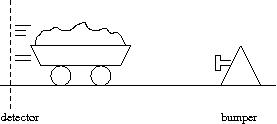
\includegraphics[width=0.4\textwidth]{carriage.jpg}
    \caption{Example: Carriage stopping before bumper.}
    \label{carriage}
\end{figure}
\end{exmp}

However, since a computer has no notion of distance, specifications in terms of physical units have to be converted to a timing constraint.
When it comes to specifications on the other hand, it's better to include the original constraint than the computed timing constraint.
This being said, the real-time programmer usually is only in charge of the computing system and cannot modify the original parameters.

Another way to classify real-time systems is by dividing them in \indexb{stand-alone systems} and systems that are \textbf{part of a hierarchy}. This course focusses on \indexb{embedded systems}: they are a component built-in to other equipment. They can either work alone or be part of a distributed system.

\begin{exmp}
An example of an \textbf{embedded system that works alone} is the electric ignition of a car, a modern washing machine or an electronic scale.
\end{exmp} 

\begin{exmp}
An example of a \textbf{embedded system that is part of a distributed system} is a network programmable controller, a programmable machine tool or more generally controllers dedicated to a component of a larger system.
\end{exmp} 


\section{Real-Time Architecture}
The classical architecture of a distributed real-time system is a two layer architecture:
\begin{enumerate}
	\item \index{Dedicated System} Dedicated System
	\item \index{Coordinating systems} Coordinating systems
\end{enumerate}

\subsection{Dedicated Controllers}
The dedicated controller usually handles tasks with critical real-time constraints. Such systems are called \indexb{hard real-time systems}. Decisions taken by the system are done so locally based on the current available information. The software's structure is simple so it offers deterministic and predictable behavior. 
 
\subsection{Central System}
The central system often deals with less critical external constraints. However, the farther remote from the controlled system, the more \textit{unpredictable events} increase the difficulty to satisfy the constraints. 
\\\\
The system centralizes information in order to provide a global view on the whole system. The operator interface is managed by this system and offers an overview of the situation, consisting of a global view and selected useful details. In a more advanced application the system might suggest actions to be undertaken by the user.

\subsection{Connections}
The connection type between the dedicated controller and the central system depends on the environment.
In an industrial environment optical fibers might be preferred to copper wires because they are not sensitive to voltage differences at the ends of the link.
Ethernet can be used on condition its behavior is deterministic.
Specialized networks exist for real-time systems (\indexb{field busses}).
Although they are not really fast they are cheap and deterministic. Either way regular traffic should be separated from the  real-time traffic of the company. 

In some cases the internal system bus of the controlling system is used instead of a network. Supplemental processors are then inserted in this bus, each with its own OS and its own memory. These processors then communicate through shared memory areas.

\subsection{System Types}
\begin{itemize}
	\item \indexb{Co\"ordinating System} (must be compatible with the external constraints)
	\begin{itemize}
		\item PC or equivalent
		\item Full fledged operating system (real-time variant of UNIX or Linux)
	\end{itemize}
	\item \indexb{Dedicated Controllers} (must be compatible with the system dedicated to)
	\begin{itemize}
		\item Programmable logic controllers
		\item Small computers with specialized operating systems
		\item Embedded Linux devices
	\end{itemize}
\end{itemize}

\subsubsection{PLC: Programmable Logic Controller}
PLCs are small computers, generally micro-controllers, executing a programmable logic controller language interpreter. The do not offer interrupts and programs are structured as a single infinite loop. At the beginning of the loop data is read, it is then processed and finally a control signal is outputted.
\\\\
The content of the loop might exist of an interpreter simulating a logic circuit. The language interpreted in then called a \indexb{ladder diagram}. Another possibility is the interpreter simulating a simple state machine. The programming language is then called \indexb{GRAFCET}. At each loop iteration a state transition is triggered based on the output of the previous state.

\paragraph{Ladder Diagram} 
The ladder diagram is a language understandable by electrical technicians. Because its expressive power is so limited manufactures have enhanced it. The PLC interprets all the lines of the diagram, which can easily span 20 or more pages, each loop. Note that if variables are used, the order of the lines become important.  

\paragraph{GRAFCET} This is a graphical language loosely inspired by PETRI nets. Rather than using logical circuits, a sequential state machine is used as a model. Although this approach is suitable for simple problems, as the problem gets more advanced, the diagram becomes equally complex.

\subsubsection{Microcomputer with Dedicated OS}
The operating system is limited but offers simple but efficient functionality:
\begin{itemize}
	\item Multitasking
	\item Fast task switching
	\item Interrupt support
	\item Inter-process communication and synchronization
\end{itemize}
Although this is more versatile than a PLC, a real programmer is needed to design the software. The more complex the software gets, the harder it becomes to guarantee response times and correctness.

\section{Time in a Real-Time System}
As mentioned in the first section, timing constraints are different for different types of systems:
\begin{itemize}
	\item \indexb{Batch processing} requires the amount of throughput, in terms of processing, to be maximized withing the available time.
	\item \indexb{Interactive systems} need short response times but only as short as the user can detect.
	\item \indexb{Real-Time systems} require the action to occur before a specific event or deadline.
\end{itemize}
Unlike the other cases, in a real-time system, the value of work does not decrease with the time needed to do the work. 

\begin{figure}[H]
    \centering
    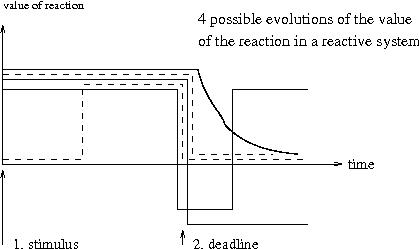
\includegraphics[width=0.6\textwidth]{reactiontime.jpg}
    \caption{Example: Time in a real-time system.}
    \label{rttime}
\end{figure}
The reaction to the stimulus (the event that triggers the response) must be performed within a certain time interval following it. (this time interval may start with the stimulus or later) During this time interval, the value of the response is constant. When the time interval is elapsed, the value of the response can:
\begin{itemize}
	\item decrease \textit{(like when cooking a soft boiled egg)}
	\item fall immediately to zero \textit{(the carriage hits the obstacle)}
	\item become negative \textit{(a hole is drilled in the printed circuit board, but at the wrong place)}
	\item become temporarily negative and then become zero\textit{ (the radar flashes the slow car driving in the right lane instead of the fast car speeding in the left lane)}
\end{itemize}

\section{Design Strategy}
When designing a real-time system the design must be as general as possible. We have to consider the hard- and software. We have to take into account the system being controlled, which is often a mechanical device and the interface between and device and the controlling system.

\begin{exmp}
By adding a simple hardware security to the controlled device, the diagram representing the value of the response in function of time can be made non-negative.
\end{exmp}

\begin{exmp}
By selecting the proper type and position of captors, the controlling system can be warned earlier and expand the acceptable reaction time span.
\end{exmp}

\begin{exmp}
Adding a DMA(Direct Memory Access) controller to the computing system makes higher rates of data acquisition possible and inversely, not adding one when none is needed makes the system cheaper.
\end{exmp}

\end{document}
